\documentclass[default,pdf,colorBG,slideColor]{prosper}
\hypersetup{pdfpagemode=FullScreen}

\usepackage{graphicx}

\title{Tor}
\subtitle{An Overview of the Second-Generation Onion Router}
\author{James Lee}
\email{jlee23@umbc.edu}
\institution{University of Maryland Baltimore County}

\begin{document}
\maketitle

\begin{slide}
~\nocite{tor-design}
\bibliographystyle{plain}
\bibliography{tor}
\end{slide}

\begin{slide}{Overview of Onion Routing}
\begin{itemize}
\item Clients choose a path through the network
\item Each node only knows the predecessor and successor nodes
\end{itemize}

\begin{center}
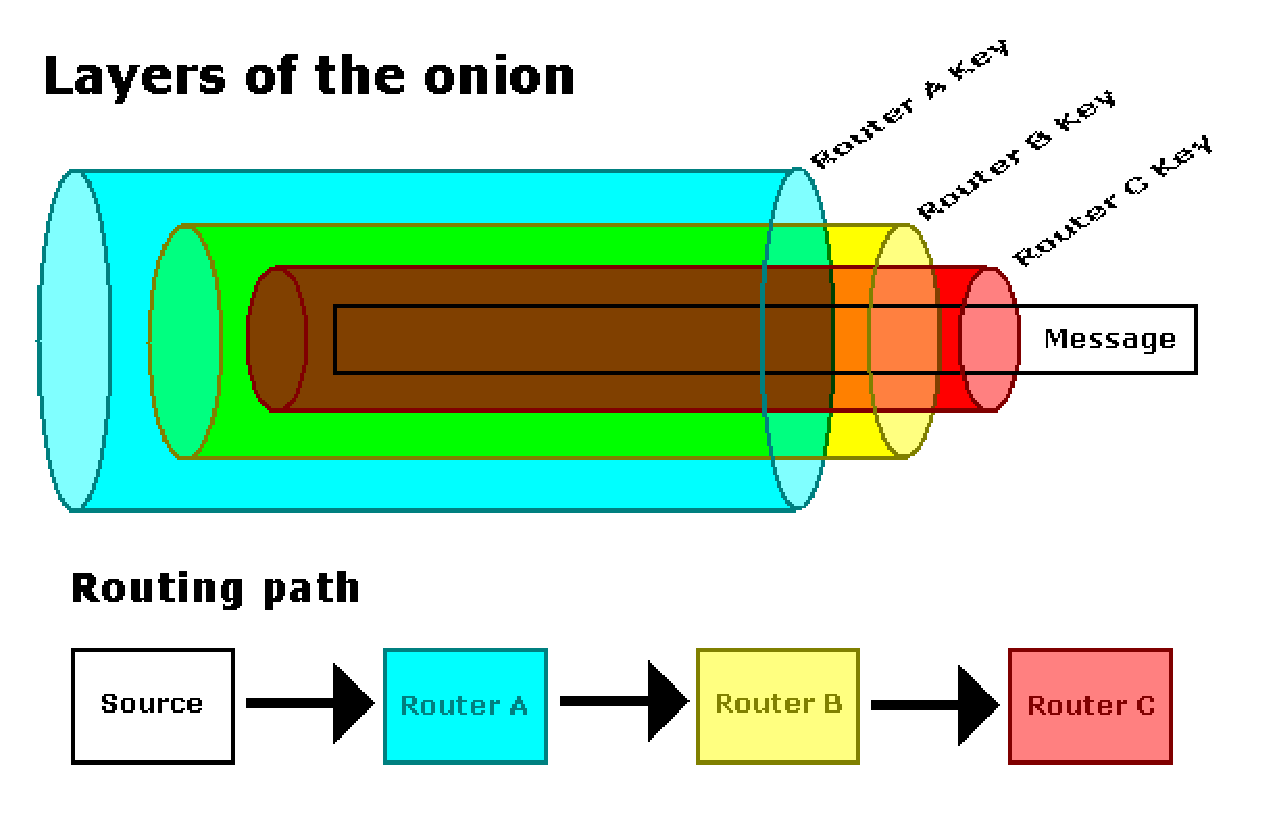
\includegraphics[width=3in]{onion.eps}
\end{center}
\end{slide}

\overlays{10}{
\begin{slide}{Improvements in Tor}
\begin{itemstep}
\item Perfect forward security
\item Separation of ``protocol cleaning'' from anonymity
\item No mixing, padding, or traffic shaping
\item Many TCP streams can share one circuit
\item Leaky-pipe circuit topology
\item Congestion control
\item Directory servers
\item Variable exit policies
\item End-to-end integrity checking
\item Rendezvous points and hidden services
\end{itemstep}
\end{slide}}

\overlays{3}{
\begin{slide}{Design Goals}
\fromSlide{1}{Above all, Tor seeks to frustrate attackers from linking communication partners.}

\begin{itemize}
\fromSlide{2}{
\item Goals
\begin{itemize}
\item Deployability
\item Usability
\item Flexibility
\item Simple Design
\end{itemize}}

\fromSlide{3}{
\item Non-goals
\begin{itemize}
\item Not peer-to-peer
\item Not secure against end-to-end attacks
\item No protocol normalization
\item Not steganographic
\end{itemize}}
\end{itemize}
\end{slide}}

\overlays{2}{
\begin{slide}{Tor Design}
\fromSlide{1}{
Overview
\begin{itemize}
\item Each onion router (OR) runs as a normal user-level process
\item Each OR maintains a TLS connection to every other OR
\item Each user runs an onion proxy (OP)
\end{itemize}}

\fromSlide{2}{
Keys
\begin{itemize}
\item Each OR has two keys: identity key and onion key
\item Identity key signs TLS certificates and router descriptions
\item Directory servers use identity keys to sign directories
\item Onion keys used to decrypt circuit setup requests
\end{itemize}}
\end{slide}}

\begin{slide}{Cells}
Cells are the basic unit of communication in Tor.

\begin{itemize}
\item ``Control'' cell:
\begin{center}
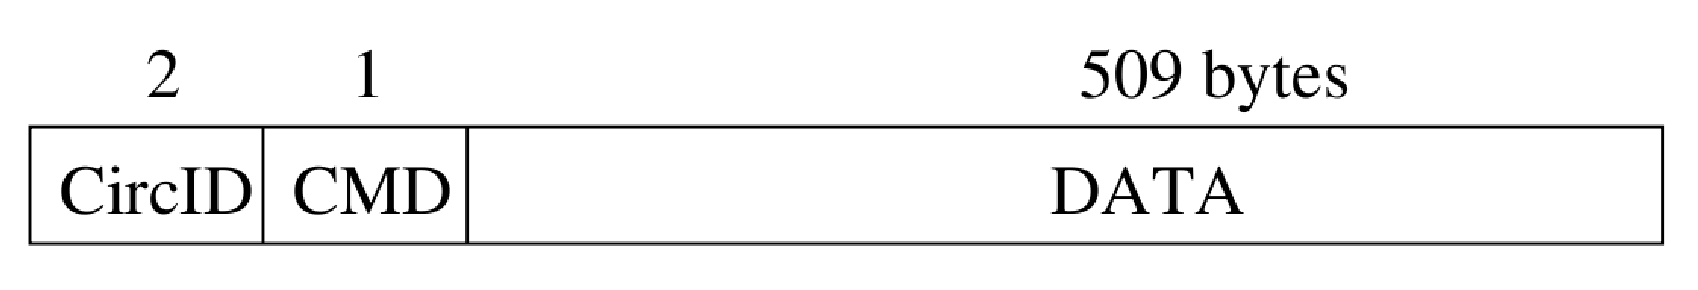
\includegraphics[width=3in]{controlcell.eps}
\end{center}

\item ``Relay'' cell:
\begin{center}
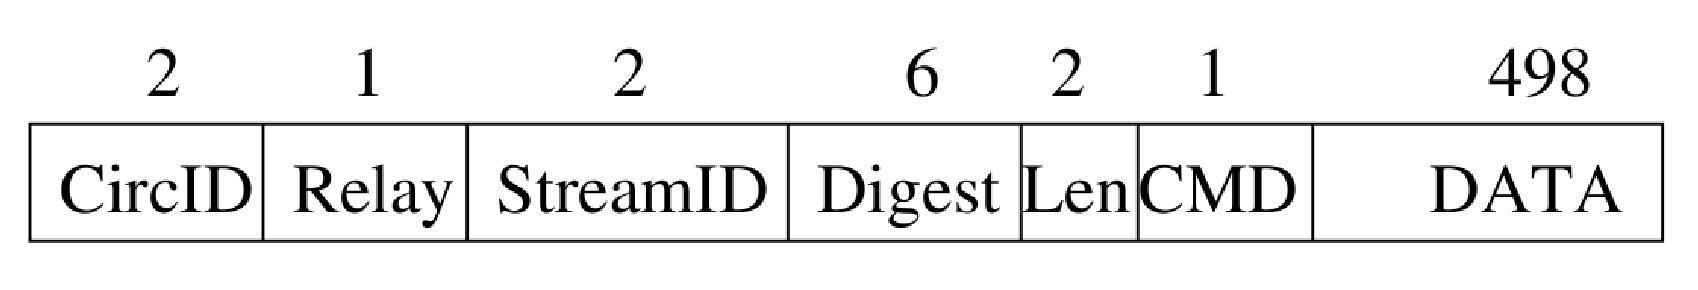
\includegraphics[width=3in]{relaycell.eps}
\end{center}
\end{itemize}
\end{slide}

\begin{slide}{Circuits and Streams}
\begin{center}
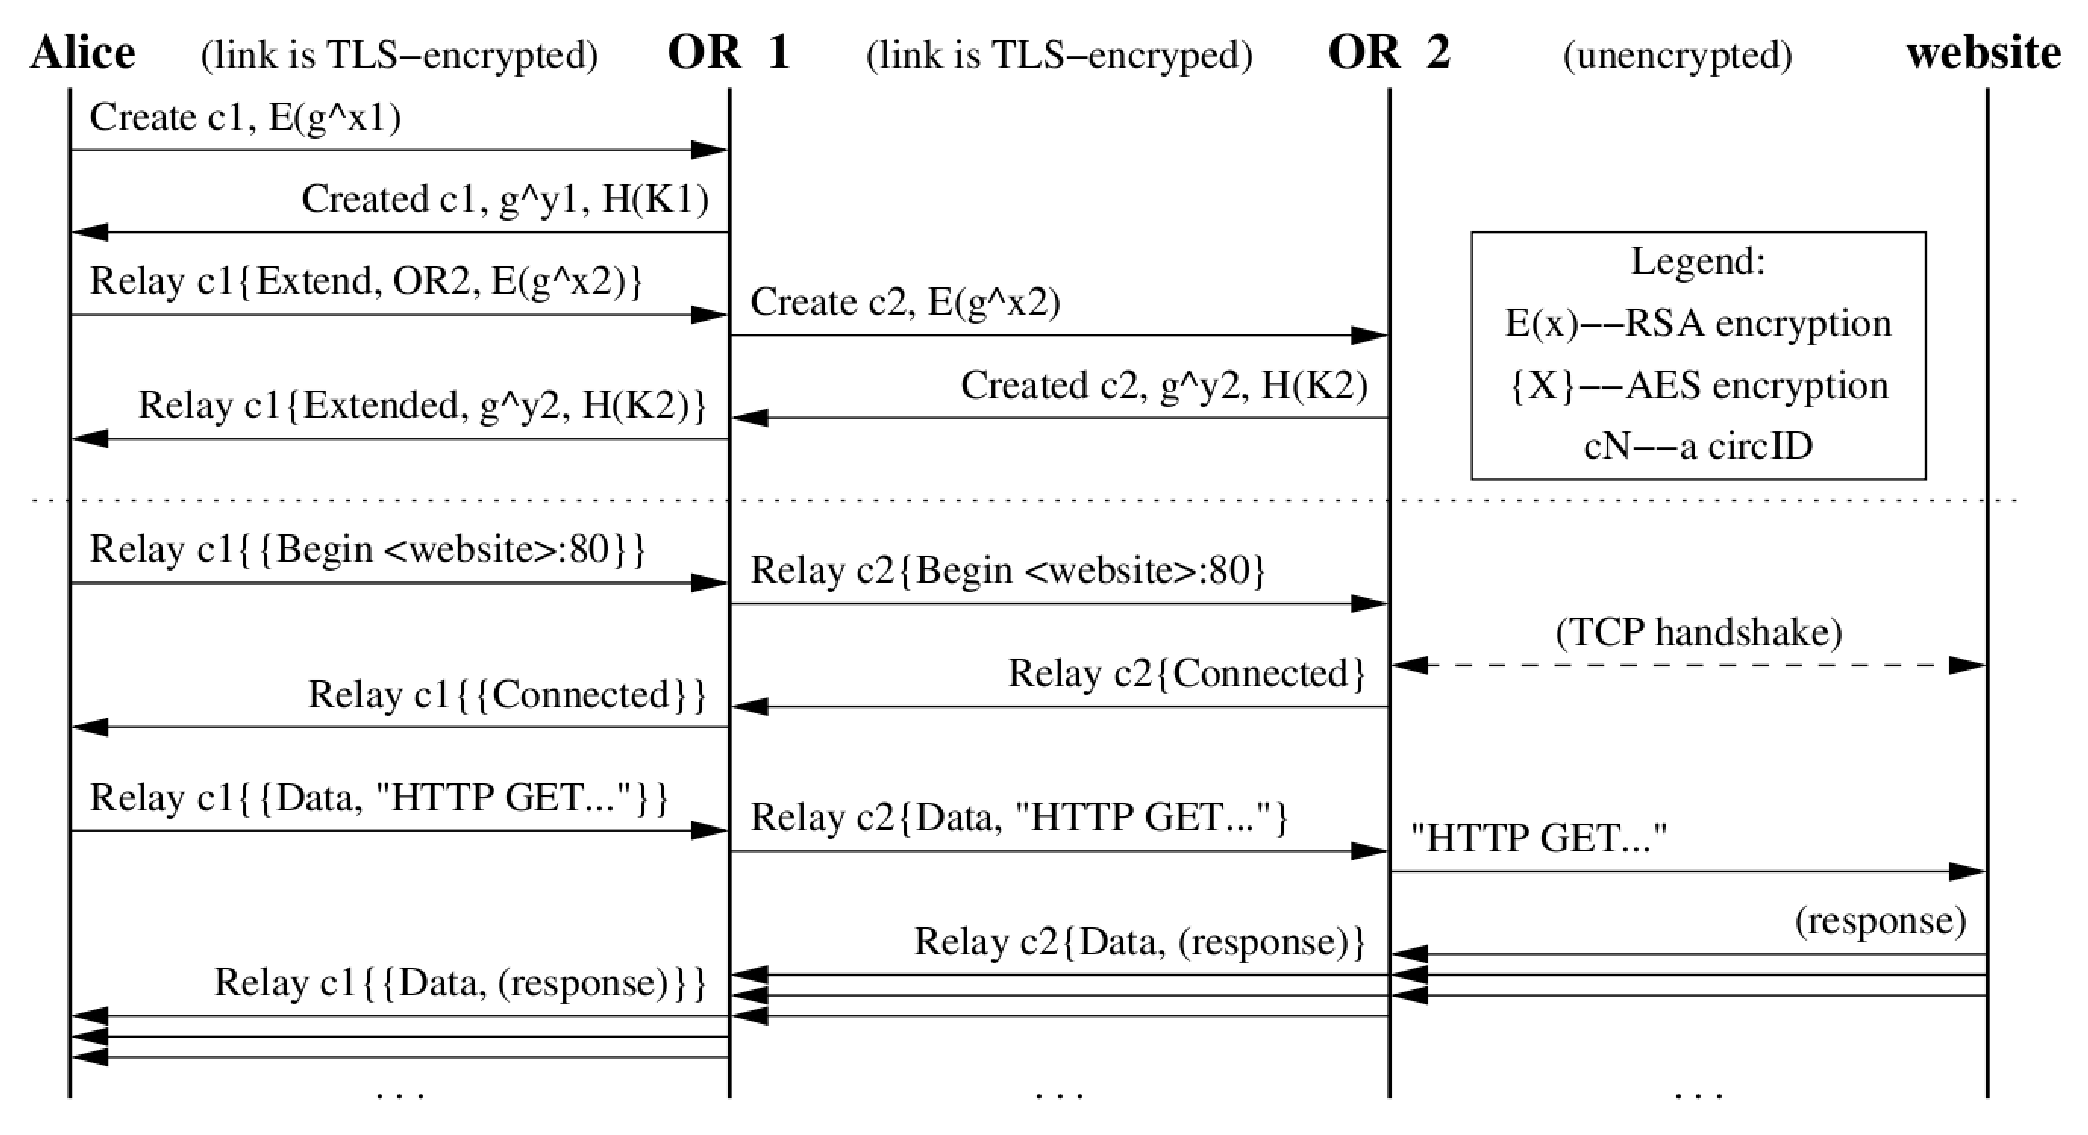
\includegraphics[width=4.5in]{circuit.eps}
\end{center}
\end{slide}
\end{document}
